% Abstract for this chapter
%
%**********************************************************************


In this chapter,
we describe motion/force control of redundant manipulators.
First, we explain the Operational Space (OS) formulation that has been traditionally used
for motion/force control and also impedance control by various researchers.
Then, we describe a new control scheme based on the Reaction Null-Space formulation.
Finally, we show the performance of the proposed method with two examples.


%%%%%%%%%%%%%%%%%%%%%%%%%
\section{Formulations}
%%%%%%%%%%%%%%%%%%%%%%%%%

%%%%%%%%%%%%%%%%%%%%%%%%%%%%%%%%%%%%%%%%%%%%
\subsection{OS formulation based control}
%%%%%%%%%%%%%%%%%%%%%%%%%%%%%%%%%%%%%%%%%%%%
From a historical point of view,
we, firstly, explain the OS formulation based motion/force control in what follows.

%
% ---------------------------------------------------------------------
\begin{figure}[t]
  \centering
  \begin{minipage}[h]{0.7\linewidth}
    \centering
    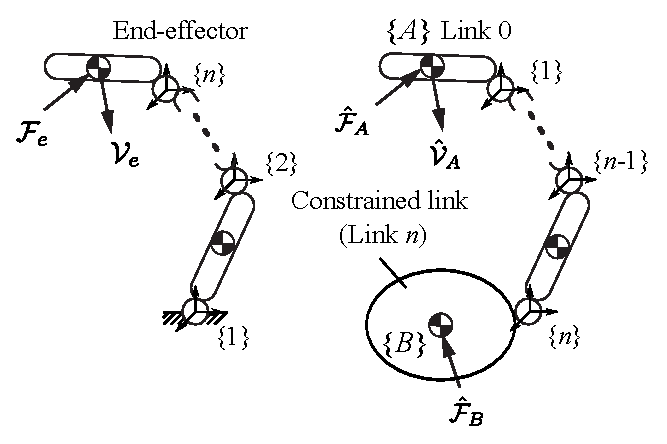
\includegraphics[width=1.0\linewidth]{fig/chapter6/models.eps}
    \footnotesize\par{Real model \hspace{8em} RNS-based control model}
  \end{minipage}
  \caption{Model of $n$-link manipulator model and its $n+1$ link control model for the RNS-based controller.}
  \label{fig:MODEL_MF}
\end{figure}
% ---------------------------------------------------------------------
%
%%%%%%%%%%%%%%%%%%%%%%%%%%%%%%%%%%%%%%%%%%%%%%%%%%%%%%%%%%%%%%
\subsubsection{Equation of motion in end-effector coordinates}
%%%%%%%%%%%%%%%%%%%%%%%%%%%%%%%%%%%%%%%%%%%%%%%%%%%%%%%%%%%%%$
Let us consider a serial $n$-link fixed base redundant manipulator as shown in the right part of \fig{MODEL_MF}.
The model has $n$-active joints and $n$-rigid body links.
We assume that the system has redundant DoF(s), i.e.\ $n > 6$.
According to the OS formulation \cite{Khatib1987},
the dynamics of a serial-link manipulator in end-effector coordinates are described
in the following form:
%
% ---------------------------------------------------------------------
\begin{align}
  \bm{M}_{e}\dot{\mathcal{V}}_{e} + \mathcal{C}_{e} + \mathcal{G}_{g} = \mathcal{F}_{e} + \mathcal{F}_{\kappa}\label{eq:EOM_EE}
\end{align}
% ---------------------------------------------------------------------
%
where $\mathcal{V}_{e}\R6$ is spatial velocity of the end-effector,
$\bm{M}_{e}\R{6 \times 6}$ defines the operational space inertia matrix and
also is reffered to as the inversion of \textit{Mobility Tensor},
$\mathcal{C}_{e}$, $\mathcal{G}_{e}\R6$ stand for Coriolis and centrifugal force and
gravity force, respectively.
$\mathcal{F}_{e}$, $\mathcal{F}_{\kappa}$ is control command with dimensions of force,
and the contact force imposed on the end-effector from enviroments.

On the other hand, because the end-effector variables
cannot become generalized coordinates of redundant manipulators,
the above equation of motion cannot be obtained directly.
Hence, a transformation is needed from the equation of motion in joint-space.

The equation of motion in joint space is  described as follows:
%
% ---------------------------------------------------------------------
\begin{align}
  \bm{M}_{l}\thdd + \bm{c}_{l} + \bm{g}_{l} = \bm{\tau} + \bm{J}_{e}^{T}\mathcal{F}_{\kappa}\label{eq:EOM_JOINT}
\end{align}
% ---------------------------------------------------------------------
%
where $\th\R{n}$ stands for the joint coordinate vector, 
$\bm{M}_{l}\R{n \times n}$ is the joint-space inertia matrix,
$\bm{c}_{l}$, $\bm{g}_{l}$ denote Coriolis and centrifugal force and
gravity force vectors in joint-space, respectively.
$\bm{\tau}\R{n}$ is joint torque vector,
$\bm{J}_{e}\R{6 \times n}$ is the Jacobian associated with the end-effector

Through the Jacobian,
the end-effector velocity/acceleration are expressed in terms of the joint variables as follows:
%
% ---------------------------------------------------------------------
\begin{align}
  \mathcal{V}_{e} &= \bm{J}_{e}\thd\label{eq:VEL_EE}\\
  \dot{\mathcal{V}}_{e} &= \bm{J}_{e}\thdd + \dot{\bm{J}}_{e}\thd\label{eq:ACC_EE}.
\end{align}
% ---------------------------------------------------------------------
%

On the other hand, from the result of statics,
end-effector force can be related to joint torque:
%
% ---------------------------------------------------------------------
\begin{align}
  \bm{\tau} = \bm{J}_{e}^{T}\mathcal{F}_{e}\label{eq:STATICS}
\end{align}
% ---------------------------------------------------------------------
%

From \eq{EOM_JOINT} to \eq{STATICS},
we can obtain the following definitions of the inertia matrix and non-linear and
gravity force vector in end-effector coordinates:
%
% ---------------------------------------------------------------------
\begin{align}
  \bm{M}_{e} &= (\bm{J}_{e}\bm{M}_{l}^{-1}\bm{J}_{e}^{T})^{-1}\\
  \mathcal{C}_{e} &= [\bm{J}_{e}^{M+}]{}^{T}\bm{c}_{l} - \bm{M}_{e}\dot{\bm{J}}_{e}\thd\\
  \mathcal{G}_{e} &= [\bm{J}_{e}^{M+}]{}^{T}\bm{g}_{l}
\end{align}
% ---------------------------------------------------------------------
%
where $\bm{J}_{e}^{M+} = \bm{M}_{l}^{-1}\bm{J}_{e}^{T}\bm{M}_{e}$ is the inertia weighted
generalized inverse of the Jacobian.

%%%%%%%%%%%%%%%%%%%%%%%%%%%%%%%%%
\subsubsection{Control command}
%%%%%%%%%%%%%%%%%%%%%%%%%%%%%%%%%
Consider now a motion/force control scenario wherein the end effector is
partially constrained by the environment.
The end-effector dynamics become
%
% ---------------------------------------------------------------------
\begin{align}
  \mathcal{F}_{e} - \bm{M}_{e}\dot{\mathcal{V}}_{e} - \mathcal{C}_{e} - \mathcal{G}_{e} = \mathcal{F}_{\kappa}
\end{align}
% ---------------------------------------------------------------------
%
To meet the control objective, a reference end-effector force is designed as
%
% ---------------------------------------------------------------------
\begin{align}
  \mathcal{F}_{e}^{ref} &= \mathcal{F}_{m}^{ref} + \mathcal{F}_{\kappa}^{ref}\label{eq:FREF_OS}\\
  \mathcal{F}_{m}^{ref} &= \bm{M}_{e}\bm{S}\dot{\mathcal{V}}_{e}^{ref} + \mathcal{C}_{e} + \mathcal{G}_{e}\\
  \mathcal{F}_{\kappa}^{ref} &= \bm{S}_{\perp}\mathcal{F}_{c}^{ref}
\end{align}
% ---------------------------------------------------------------------
%
where $\mathcal{F}_{m}^{ref}$ and $\mathcal{F}_{\kappa}^{ref}$ are two components referring to
end-effector motion and contact force, respectively.
$\bm{S}\R{6 \times 6}$ is a selection matrix suitably defined to specify the unconstrained motion direction,
while $\bm{S}_{\perp}\R{6 \times 6}$ is its complement.
$\dot{\mathcal{V}}_{e}^{ref}$ and $\mathcal{F}_{c}^{ref}$ are reference value for the motion and
force tasks, respectively,
that usually involve feedback control terms.

Further on, since the manipulator is redundant, there is an infinite set of control joint torques
that could be applied without affecting the resultant forces at the end-effector \cite{Khatib1987}.
%
% ---------------------------------------------------------------------
\begin{align}
  \bm{\tau} = \bm{J}_{e}^{T}\mathcal{F}_{e}^{ref} + (\bm{E} - \bm{J}_{e}^{T}\bm{J}_{e}^{M+})\bm{\tau}_{a}\label{eq:TAU_OS1}
\end{align}
% ---------------------------------------------------------------------
%
where $(\bm{E} - \bm{J}_{e}^{T}\bm{J}_{e}^{M+})$ denotes a projector onto the null-space of the transposed
inertia -weighted generalized inverse of the Jacobian, $\bm{E}$ standing for
the $n \times n$ identity matrix.
$\bm{\tau}_{a}$, an arbitrary joint torque vector,
parametrizes (in a non-minimal way) the set of joint torques that do not impose
any end-effector force.
Moreover, there is also another infinite set of control joint torques that produce the same
end-effector acceleration as a given end-effector force:
%
% ---------------------------------------------------------------------
\begin{align}
  \bm{\tau} = \bm{M}_{l}\bm{J}^{\#}\bm{M}_{e}^{-1}\mathcal{F}_{e}^{ref} +
  \bm{M}_{l}(\bm{E} - \bm{J}_{e}^{\#}\bm{J}_{e})\thdd_{a}\label{eq:TAU_OS2}
\end{align}
% ---------------------------------------------------------------------
%
where $\thdd_{a}\R{n}$ stands for an arbitrary joint acceleration vector,
$(\circ)^{\#}$ denotes generalized inverse of the corresponding matrix.
The two joint-torque sets \eq{TAU_OS1} and \eq{TAU_OS2} are compatible (or dynamically consistent),
only when the inertia-weighted generalized inverse of the Jacobian is applied in \eq{TAU_OS2}.
This leads to \textit{complete dynamic decoupling} between the particular components
responsible for the motion/force control task and the null-space components.

The property of complete dynamic decoupling plays an important role in motion/force
and impedance control design, since task and null-space control components can be designed
independently.
However, the nominal behavior in joint space determined by the task-space control component
may become unstable due to ill-conditioning of the inertia weighted generalized inverse.
Also, the joint velocity may grow in an uncontrollable fashion because of the non-integrability of
joint acceleration. Although these problems can be alleviated via the null-space control component,
it would be much more desirable to have a controller with a satisfactory nominal behavior.

% %%%%%%%%%%%%%%%%%%%%%%%%%%%%%%%%%%%%%%%%%%%%%%%%%%%%
% \subsubsection{Problem in the gravity compensation}
% %%%%%%%%%%%%%%%%%%%%%%%%%%%%%%%%%%%%%%%%%%%%%%%%%%%%



%%%%%%%%%%%%%%%%%%%%%%%%%%%%%%%%%%%%%%%%%%%%%%%%%%
\subsection{Reaction Null-Space based control}
%%%%%%%%%%%%%%%%%%%%%%%%%%%%%%%%%%%%%%%%%%%%%%%%%%
In what follows, we describe the RNS-based motion/force control for fixed-base redundant manipulators.

%%%%%%%%%%%%%%%%%%%%%%%%%%%%%%%%%%%%%%%%%%%%%%%%%%%%%%%%%%%%%%%%%%%%%%%%%%
\subsubsection{End-link dynamics based on free-floating base coordinates}
%%%%%%%%%%%%%%%%%%%%%%%%%%%%%%%%%%%%%%%%%%%%%%%%%%%%%%%%%%%%%%%%%%%%%%%%%%
For the RNS based motion/force control,
we consider a free-floating base serial-link manipulator with $n+1$ links, as shown in the right part of \fig{MODEL_MF}.
The two end-links are denoted as $A$ and $B$.
Without loss of generality, in what follows end-link $A$ will be designed as the root link.
It is convenient to assume that the root link is connected to the inertial frame via a virtual six-DoF joint.
Hence, there are $n+6$ generalized coordinates:
the $n$ joint coordinated plus 
the six coordinates of the root end-link $A$.
There are three points of interest:
characteristic points on each of the two end-links (points $A$ and $B$ in \fig{MODEL_MF})
and the total center of mass.
External spatial forces $\hmathc{F}_{A}$ and $\hmathc{F}_{B}$ act at points $A$ and $B$, respectively.
The motion of the two end-links is characterized by spatial velocities $\hmathc{V}_{A}$ and $\hmathc{V}_{B}$.
Note that we distinguish the quantities of RNS based control model from these of the real model
through the notation $\hat{(\circ)}$.

The system dynamics are described by two coupled equations:
%
% ---------------------------------------------------------------------
\begin{align}
  \hbm{M}_{A}\dot{\hmathc{V}}_{A} + \hbm{M}_{Al}\hthdd + \hmathc{C}_{A} + \hmathc{G}_{A} &=
  \hmathc{F}_{A} + \hbm{T}\hmathc{F}_{B}\label{eq:EOM_MF_TASK}\\
  \hbm{M}_{Al}^{T}\dot{\hmathc{V}}_{A} + \hbm{M}_{l}\hthdd + \hbm{c}_{l} \hbm{g}_{l} &=
  \hbm{\tau} + \hbm{J}_{B}^{T}\hmathc{F}_{B}\label{eq:EOM_MF_JOINT}
\end{align}
% ---------------------------------------------------------------------
%
First, note that in \eq{EOM_MF_TASK} three are two linear force components.
$\hbm{M}_{Al}\hthdd$ reflects the inertial coupling between end-link $A$ and the rest of the links.
Component $\hbm{M}_{A}\dot{\hmathc{V}}_{A}$, on the other hand,
represents the inertia force of the composite rigid body (CRB) obtained when the joints are momentarily locked.
The CRB dynamics are characterized by the inertial properties of the entire system;
they are represented in terms of end-link $A$ coordinates.

Next, note that \eq{EOM_MF_JOINT} would represent the dynamics of a ``conventional'' fixed-base manipulator,
where link $A$ is fixed.
This manipulator is composed of all bodies except link $A$;
because end-link $A$ is the root, quantities $\hbm{M}_{l}$, $\hbm{c}_{l}$, $\hbm{g}_{l}$ and
$\hbm{J}_{B}$ are those of the fixed-base manipulator, link $B$ being its end-effector.
To adapt this floating-base notation to the fixed-base manipulator described above,
we will keep end-link $A$ as the root link, but designate it as the end-effector.
End link $B$, on the other hand,
will be fully constrained to become the fixed base.
This implies the renumbering of joints and links in reverse order, as illustrated in \fig{MODEL_MF}.

%%%%%%%%%%%%%%%%%%%%%%%%%%%%%%%%%%
\subsubsection{Control command}
%%%%%%%%%%%%%%%%%%%%%%%%%%%%%%%%%%
Our goal is to design a controller with a task-space control component that can ensure the desirable
nominal behavior in joint space,
such that large joint-velocity peaks and velocity build-up can be avoided.
The derivation is based on the hybrid motion/force control approach presented in \cite{Siciliano2008}.
End-effector $A$ contacts the environment under a motion/force task scenario,
being thereby constrained along $k < 6$ directions.
This can be expressed via the equation $\hbm{J}_{\kappa}(\hqd)\hqd = \bm{0}$,
$\hbm{J}_{\kappa}(\hqd)\R{k \times (6+\kappa)}$ denoting the constraint Jacobian containing
partial derivatives related to the environment constraint $\bm{\kappa}(\hqd) = \mathrm{const}$.
End-effector $A$'s spatial force is then $\hmathc{F}_{A} = \hbm{J}_{\kappa A}^{T}\hbm{\lambda}$,
where $\hbm{\lambda}\R{k}$ is the Lagrange multiplier for the forces of constraint and
$\hbm{J}_{\kappa A}(\hqd)\R{k \times 6}$ is a submatrix of
the constraint Jacobian s.t.\ $\hbm{J}_{\kappa A}\hmathc{V}_{A} = \bm{0}$.
Further on, denote $\hmathc{V}_{A} = \hbm{S}_{v}\hbm{\nu}_{A}$ where $\hbm{\nu}_{A}$ is end-effector $A$'s
velocity along the unconstrained directions and $\hbm{S}_{v}(\hq)$ is defined from $\hbm{S}_{f}^{T}\hbm{S}_{v} = \bm{0}$,
$\hbm{S}_{f} = \hbm{J}_{\kappa A}^{T}(\hq)$.

Using \eq{EOM_MF_TASK}, we first obtain the reference joint
acceleration for the task-space (particular-solution) control component:
%
% ---------------------------------------------------------------------
\begin{align}
  \hthdd = \hbm{M}_{Al}^{+}(\hbm{S}_{f}\hbm{f}_{\lambda} - \hbm{M}_{A}\hbm{S}_{v}\hbm{\alpha}_{v} - \hbm{M}_{A}\dot{\hbm{S}}_{v}\hbm{\nu})
  + \hbm{M}_{Al}^{+}(\hbm{T}\hmathc{F}_{B} - \hmathc{C}_{B} - \hmathc{G}_{B})\label{eq:THDD_REF_RNS}
\end{align}
% ---------------------------------------------------------------------
%
This control acceleration ensures complete decoupling between the motion and force subtasks for the closed-loop system.
The respective joint torque control component derived via \eq{EOM_MF_JOINT} is
%
% ---------------------------------------------------------------------
\begin{align}
  \hbm{\tau}^{ref} =  (&\hbm{M}_{Al}^{T} - \hbm{M}_{l}\hbm{M}_{Al}^{+}\hbm{M}_{A})\hbm{S}_{v}\hbm{\alpha}_{v} +
  \hbm{M}_{l}\hbm{M}_{Al}^{+}\hbm{S}_{f}\hbm{f}_{\lambda}\notag\\
  &+ (\hbm{M}_{l}\hbm{M}_{Al}^{+}\hbm{T} - \hbm{J}_{B}^{T})\hmathc{F}_{B}\notag\\
  &+ \hbm{c}_{l} + \hbm{g}_{l} - \hbm{M}_{l}\hbm{M}_{Al}^{+}(\hmathc{C}_{A} + \hmathc{G}_{A} + \hbm{M}_{A}\dot{\hbm{S}}_{v}\hbm{\nu})\label{eq:TAU_REF_RNS}
\end{align}
% ---------------------------------------------------------------------
%
This control torque compensates the joint-space non-linear and gravity forces and ensures a double-integrator type
closed-loop behavior $\hthdd = \hthdd^{ref}$.
When compared to the particular-solution control torque derived under the OS formulation,
$\bm{\tau} = \bm{J}_{e}^{T}\mathcal{F}_{e}^{ref}$,
$\mathcal{F}_{e}^{ref}$ given in \eq{FREF_OS},
the above expression is somewhat messier.
But we can expect a better nominal behavior in joint-space, as explained.
The following remarks are due.
First, note that with the controller we have to compensate the exact non-linear force term $\hmathc{C}_{A}$ instead of
compensating its approximation $\hmathc{C}_{A} \approx \dot{\hbm{M}}_{A}\hmathc{V}_{A} + \hbm{M}_{Al}\hthd$
that was required for momentum conservation;
otherwise, the task-space behavior cannot be guaranteed anymore.


%%%%%%%%%%%%%%%%%%%%%%%%%%%%%%
\subsubsection{Constraint force}
%%%%%%%%%%%%%%%%%%%%%%%%%%%%%%
To implement the RNS-based control,
a constraint force that makes the link $B$ the fixed base has to be presented.
The constraint force is obtained through the method of Lagrange multiplier in what follows.

First, we obtain the kinematic equation of the constrained link velocity as follows:
% 
% ---------------------------------------------------------------------
\begin{align}
  \hat{\mathcal{V}}_{B} &= \hbm{T}^{T}\hat{\mathcal{V}}_{A} + \hbm{J}_{B}\hthd \notag\\
  &= \hbm{J}_{const}\hqd
\end{align}
% ---------------------------------------------------------------------
%
where $\hbm{J}_{const} = [\hbm{T}~\hbm{J}]\R{6 \times (n+6)}$ stands for constraint Jacobian,
$\qd = [\mathcal{V}_{A}^{T}~\thd^{T}]^{T}$ denotes the generalized velocity vector.
Since the condition of fixed base is $\mathcal{V}_{B} = \bm{0}$,
the following equation, hence, has to be satisfied:
% 
% ---------------------------------------------------------------------
\begin{align}
  \hbm{J}_{const}\hqdd + \dot{\hbm{J}}_{const}\hqd = \bm{0}\label{eq:CONST_MF}
\end{align}
% ---------------------------------------------------------------------
%

On the other hand,
the equation of motion of the control model can be expressed in the following compact form:
%
% ---------------------------------------------------------------------
\begin{align}
  \hat{\bm{M}}\qdd + \hat{\bm{c}} + \hat{\bm{g}} = \hat{\bm{Q}} + \hbm{J}_{const}^{T}\hat{\mathcal{F}}_{B}\label{eq:EOM_MF_COMP}
\end{align}
% ---------------------------------------------------------------------
%
Then, substituting \eq{EOM_MF_COMP} into \eq{CONST_MF} and solving it for $\hat{\mathcal{F}}_{B}$,
we can obtain the constraint force as follows:
%
% ---------------------------------------------------------------------
\begin{align}
  \hat{\mathcal{F}}_{B} = (\hbm{J}_{const}\hbm{M}^{-1}\hbm{J}_{const}^{T})^{-1}\Big(\hbm{J}_{const}\hbm{M}^{-1}(\hbm{c} + \hbm{g} - \hbm{Q})
  - \dot{\hbm{J}}_{const}\hqd\Big)
\end{align}
% ---------------------------------------------------------------------
%
Finally, the constraint force is substituting into \eq{THDD_REF_RNS} and \eq{TAU_REF_RNS}.


% %%%%%%%%%%%%%%%%%%%%%%%%%%%%%%%%%%%%%%%%%%%%%%%%%%%%%%%%%%%%%%%%%%%%%%%%%%%%%%%%%%%%%%%
% \subsection{Parameter transformation between a real model and a control model}
% %%%%%%%%%%%%%%%%%%%%%%%%%%%%%%%%%%%%%%%%%%%%%%%%%%%%%%%%%%%%%%%%%%%%%%%%%%%%%%%%%%%%%%%

%%%%%%%%%%%%%%%%%%%%%
\section{Examples}
%%%%%%%%%%%%%%%%%%%%%

%%%%%%%%%%%%%%%%%%%%%%%%%%%%%%%%%%%%%%%%%%%%
\subsection{Planar three-DoF manipulator}
%%%%%%%%%%%%%%%%%%%%%%%%%%%%%%%%%%%%%%%%%%%%
%
% ---------------------------------------------------------------------
\begin{figure}[t]
  \centering
  \begin{minipage}{0.8\linewidth}
    \centering
    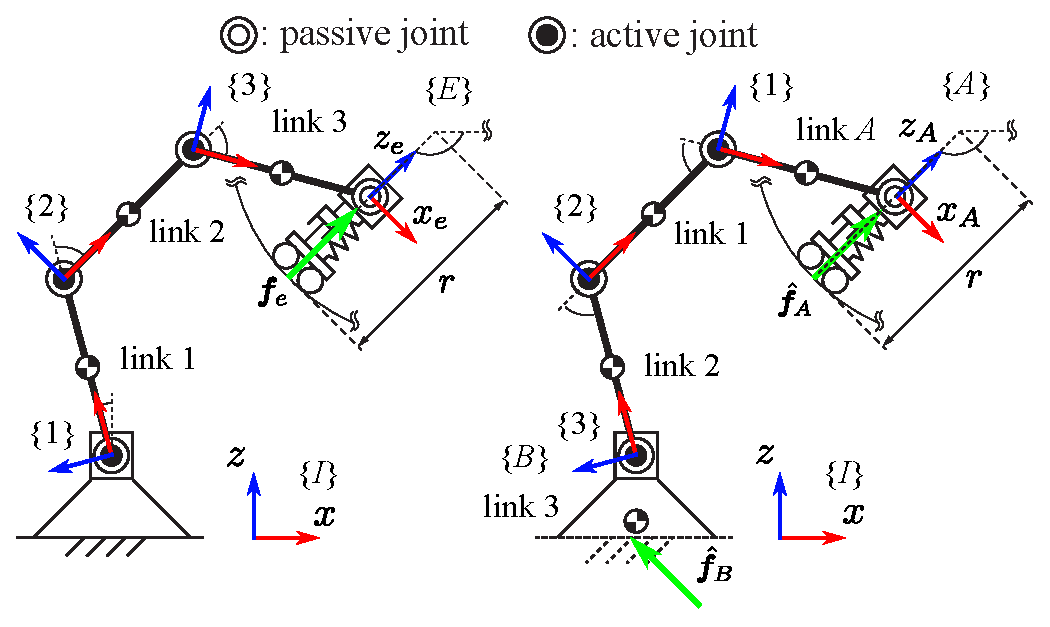
\includegraphics[width=1.0\linewidth]{fig/chapter6/3Rmani.eps}
    \footnotesize\par{\hspace{-20mm}(a)\hspace{70mm}(b)}
  \end{minipage}
  \caption{Three-link planar redundant manipulator: (a) real model and (b) control model.}
  \label{fig:3R_MANI}
\end{figure}
% ---------------------------------------------------------------------
%
In what follows, we provide two examples to evaluate the performance of the proposed control.
First, we consider a planar three-DoF redundant manipulator as shown in \fig{3R_MANI}~(a).
We assume that the end-effector contacts with an environment at a point.
Contact force acting to the end-effector has only force component;
the moment of force component is ignored.
And also the end-effector orientation is not considered here.
Hence, the system has one degree-of-redundancy.

The control model for the RNS based control is displayed in \fig{3R_MANI}~(b).
As shown in the figure,
link 3 of the control model is regarded as the constrained link.
The equation of motion of the control model is described as follows:
%
% ---------------------------------------------------------------------
\begin{align}
  \bmat{\hbm{M}_{v} & \hbm{M}_{v\omega} & \hbm{M}_{vl}\\
    \hbm{M}_{v\omega}^{T} & \hat{M}_{\omega} & \hbm{M}_{\omega l}\\
    \hbm{M}_{vl}^{T} & \hbm{M}_{\omega l}^{T} & \hbm{M}_{l}}
  \bmat{\hbm{v}_{A} \\ \hat{\omega}_{A} \\ \hthdd}
  +
  \bmat{\hbm{c}_{v_{A}} \\ \hat{c}_{\omega_{A}} \\ \hbm{c}_{l}}
  +
  \bmat{\hbm{g}_{v_{A}} \\ \hat{g}_{\omega_{A}} \\ \hbm{g}_{l}}
  =
  \bmat{\hbm{f}_{A} \\ 0 \\ \hbm{\tau}}
  +
  \bmat{\hbm{T} \\ \hbm{J}_{B}}\bmat{\hbm{f}_{B} \\ \hat{n}_{B}}
  \label{eq:EOM_MF_3R}
\end{align}
% ---------------------------------------------------------------------
%
where the dimension of each coordinate are $\hat{\bm{v}}_{A}\R2$,
$\hat{\omega}_{A}$ and $\hthdd\R3$.
Then, the size of the matrices is determined according to the dimension of the coordinate variables.
Because we assume end-effector linear motion only,
the equation of motion has to be modified.
First, estimated from the middle part of \eq{EOM_MF_3R},
the angular acceleration of link $A$ can be obtained as follows:
%
% ---------------------------------------------------------------------
\begin{align}
  \dot{\hat{\omega}}_{A} = -\hat{M}_{\omega}^{-1}(\hbm{M}_{v\omega}^{T}\dot{\hbm{v}}_{A} + \hbm{M}_{\omega l}\hthdd + \hat{c}_{\omega_{A}}
  + \hat{g}_{\omega_{A}} - \hbm{T}_{\omega}\bmat{\hbm{f}_{B}^{T} & \hat{n}_{B}}^{T})\label{eq:3R_ROT}
\end{align}
% ---------------------------------------------------------------------
%
where $\hbm{T}_{\omega}\R{1 \times 3}$ is the pose matrix associated with rotation.
Then, substituting \eq{3R_ROT} into the upper part of \eq{EOM_MF_3R},
we can obtain the following equation of motion with reduced form:
%
% ---------------------------------------------------------------------
\begin{align}
  (\hbm{M}_{v} - \hbm{M}_{v\omega}\hat{M}_{\omega}^{-1}\hbm{M}_{v\omega}^{T})\ddot{\hbm{v}}_{A} +
  (\hbm{M}_{vl} - \hbm{M}_{v \omega}\hat{M}_{\omega}^{-1}\hbm{M}_{\omega l})\hthdd +\notag\\
  (\hbm{c}_{v_{A}} - \hbm{M}_{v\omega}\hat{M}_{\omega}\hat{c}_{\omega_{A}}) +
  (\hbm{g}_{v_{A}} - \hbm{M}_{v\omega}\hat{M}_{\omega}\hat{g}_{\omega_{A}})\notag\\
  = (\hbm{T}_{v} - \hbm{M}_{v\omega}\hat{M}_{\omega}^{-1}\hbm{T}_{\omega})\bmat{\hbm{f}_{B}^{T} & \hat{n}_{B}}^{T}
\end{align}
% ---------------------------------------------------------------------
%
Then, the reference joint acceleration can be obtaind as:
%
% ---------------------------------------------------------------------
\begin{align}
  \hthdd^{ref} =   (\hbm{M}_{vl} - \hbm{M}_{v \omega}\hat{M}_{\omega}^{-1}\hbm{M}_{\omega l})^{+}\Big\{
  (\hbm{M}_{v} - \hbm{M}_{v\omega}\hat{M}_{\omega}^{-1}\hbm{M}_{v\omega}^{T})\ddot{\hbm{v}}_{A}^{ref} +\notag\\
  (\hbm{c}_{v_{A}} - \hbm{M}_{v\omega}\hat{M}_{\omega}\hat{c}_{\omega_{A}}) +
  (\hbm{g}_{v_{A}} - \hbm{M}_{v\omega}\hat{M}_{\omega}\hat{g}_{\omega_{A}})\notag\\
  - (\hbm{T}_{v} - \hbm{M}_{v\omega}\hat{M}_{\omega}^{-1}\hbm{T}_{\omega})\bmat{\hbm{f}_{B}^{T}{}^{ref} & \hat{n}_{B}}^{T}\Big\}
\end{align}
% ---------------------------------------------------------------------
%



%%%%%%%%%%%%%%%%%%%%%%%%%%%%%%%%%%%%%%%%%%
\subsubsection{Parameter transformation}
%%%%%%%%%%%%%%%%%%%%%%%%%%%%%%%%%%%%%%%%%%
Under the RNS-based motion/force controller,
we have to consider the relations of model parameters between the two models.
End-effector coordinates, joint coordinate and joint torque are transformed according to
the following relations:
%
% ---------------------------------------------------------------------
\begin{align}
   [\hat{x}_{A}~\hat{z}_{A}~\hat{\psi}_{A}]^{T} &= [x_{e}~z_{e}~\psi_{e}]^{T}\\
   [\hat{\theta}_{1}~\hat{\theta}_{2}~\hat{\theta}_{3}]^{T} &= -[\theta_{3}~\theta_{2}~\theta_{1}]^{T}\\
   [\hat{\tau}_{1}~\hat{\tau}_{2}~\hat{\tau}_{3}]^{T} &= -[\tau_{3}~\tau_{2}~\tau_{1}]^{T}
\end{align}
% ---------------------------------------------------------------------
%
In addition,
the model parameters, such as link length, mass and inertia moment,
are determined as follows:
%
% ---------------------------------------------------------------------
\begin{align}
  [\hat{l}_{A}~\hat{l}_{1}~\hat{l}_{2}~\hat{l}_{3}]^{T} &= [l_{3}~l_{2}~l_{1}~\hat{l}_{3}]^{T}\\
  [\hat{m}_{A}~\hat{m}_{1}~\hat{m}_{2}~\hat{m}_{3}]^{T} &= [m_{3}~m_{2}~m_{1}~\hat{m}_{3}]^{T}\\
  [\hat{I}_{A}~\hat{I}_{1}~\hat{I}_{2}~\hat{I}_{3}]^{T} &= [I_{3}~I_{2}~I_{1}~\hat{I}_{3}]^{T}
\end{align}
% ---------------------------------------------------------------------
%
Note that the parameters of link 3 do not have a physical meaning
because there is no corresponding part in the real model.
Hence, these can be arbitrary values.

%%%%%%%%%%%%%%%%%%%%%%%%%%
\subsubsection{Simulation}
%%%%%%%%%%%%%%%%%%%%%%%%%%

%
% ---------------------------------------------------------------------
\begin{figure}[t]
  \centering
  \begin{minipage}[h]{0.40\linewidth}
    \centering
    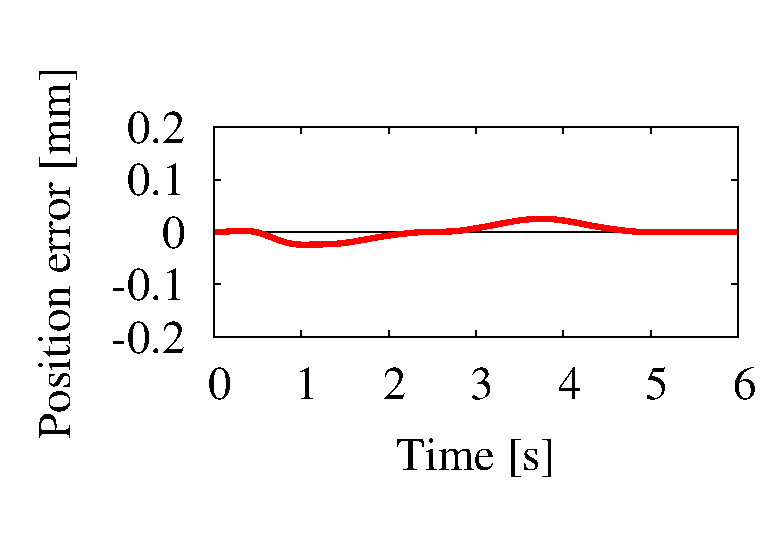
\includegraphics[width=1.0\linewidth]{fig/chapter6/results/planar/RNS/3RFIX_RNS_U06_pos_err.eps}
  \end{minipage}
  \begin{minipage}[h]{0.40\linewidth}
    \centering
    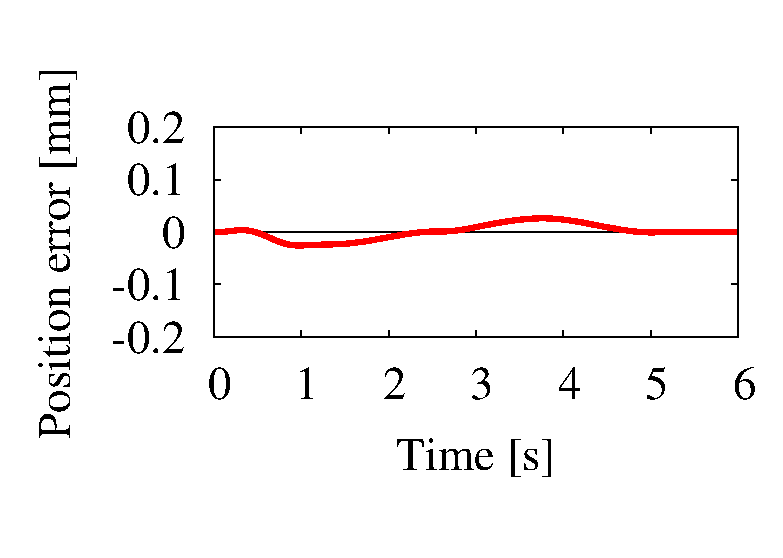
\includegraphics[width=1.0\linewidth]{fig/chapter6/results/planar/OSF/3RFIX_OSF_U06_pos_err.eps}
  \end{minipage}\\
  \vspace{-7mm}
  \begin{minipage}[h]{0.40\linewidth}
    \centering
    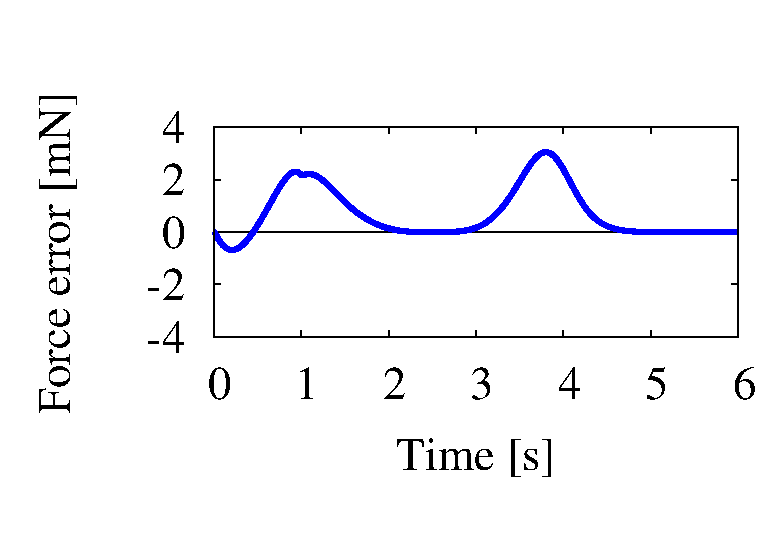
\includegraphics[width=1.0\linewidth]{fig/chapter6/results/planar/RNS/3RFIX_RNS_U08_force_err.eps}
  \end{minipage}
  \begin{minipage}[h]{0.40\linewidth}
    \centering
    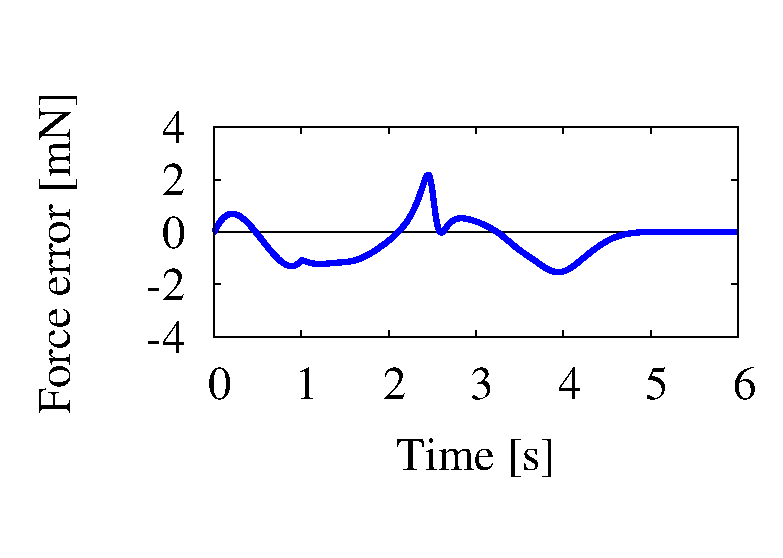
\includegraphics[width=1.0\linewidth]{fig/chapter6/results/planar/OSF/3RFIX_OSF_U08_force_err.eps}
  \end{minipage}
  \footnotesize\par{RNS-C \hspace{13em} OS-C}
  \vspace{1em}
  \caption{Simulation results of end-effector position and force.
  The position error is along $x$-direction, while the force error is represented along $z$ direction,
  in the end-effector frame.}
  \label{fig:RES_MF_3R_TASK}
\end{figure}
% ---------------------------------------------------------------------
%
%
% ---------------------------------------------------------------------
\begin{figure}[t]
  \centering
  \begin{minipage}[h]{0.40\linewidth}
    \centering
    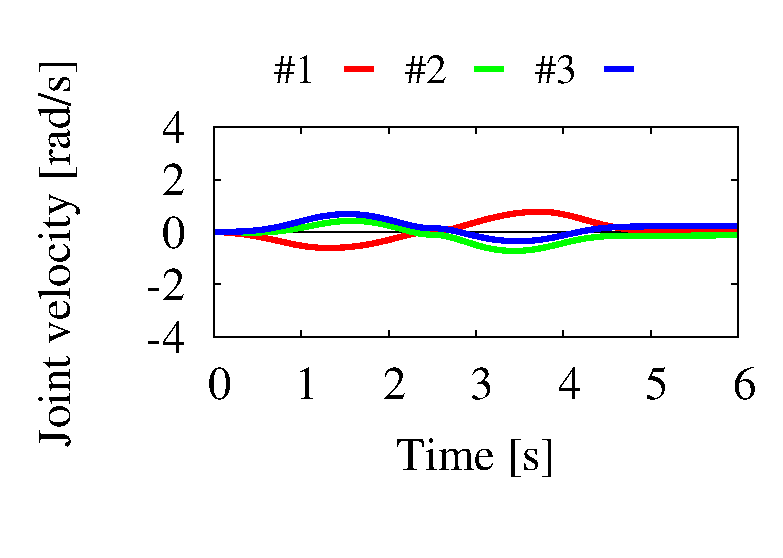
\includegraphics[width=1.0\linewidth]{fig/chapter6/results/planar/RNS/3RFIX_RNS_X02_Joint_velo.eps}
  \end{minipage}
  \begin{minipage}[h]{0.40\linewidth}
    \centering
    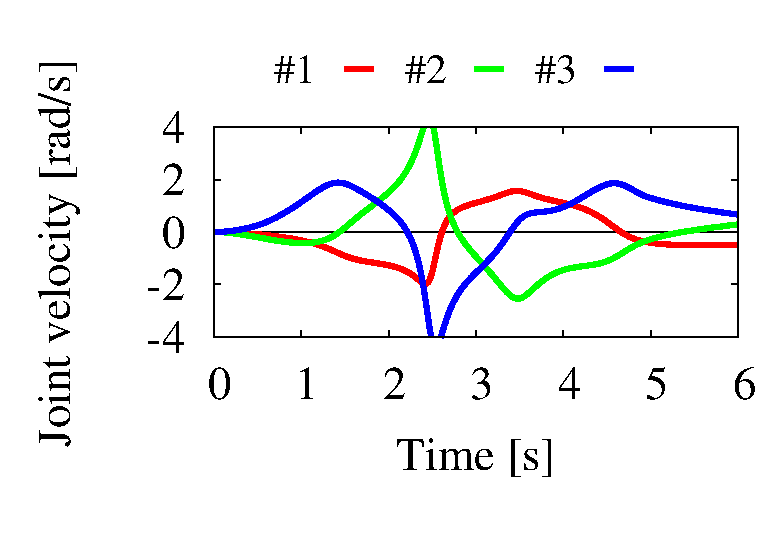
\includegraphics[width=1.0\linewidth]{fig/chapter6/results/planar/OSF/3RFIX_RNS_X02_Joint_velo.eps}
  \end{minipage}\\
  \vspace{-5mm}
  \begin{minipage}[h]{0.40\linewidth}
    \centering
    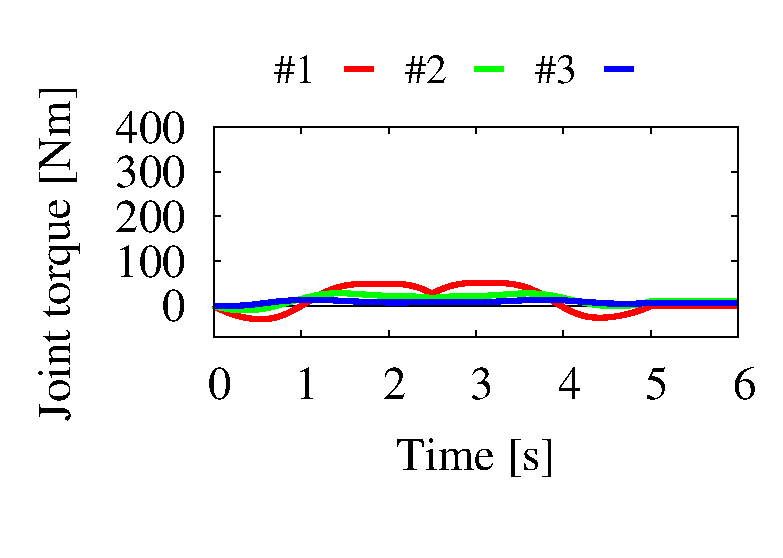
\includegraphics[width=1.0\linewidth]{fig/chapter6/results/planar/RNS/3RFIX_RNS_U01_torque.eps}
  \end{minipage}
  \begin{minipage}[h]{0.40\linewidth}
    \centering
    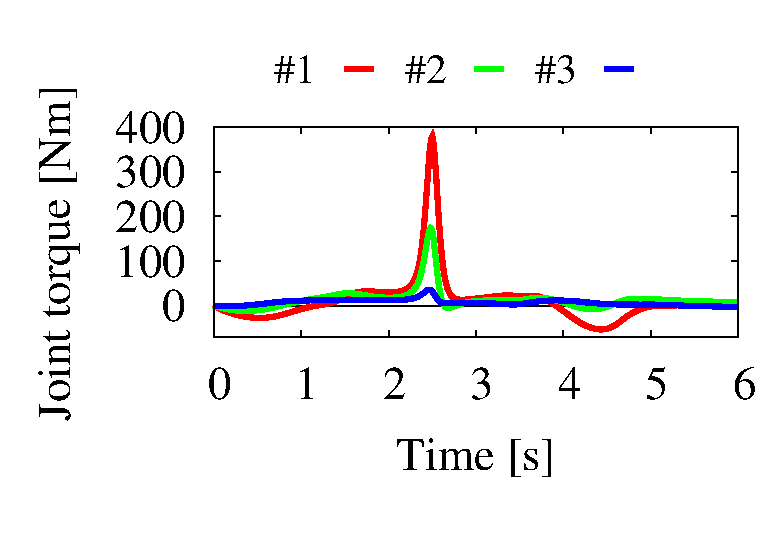
\includegraphics[width=1.0\linewidth]{fig/chapter6/results/planar/OSF/3RFIX_OSF_U01_torque.eps}
  \end{minipage}\\
  \footnotesize\par{RNS-C \hspace{13em} OS-C}
  \vspace{1em}
  \caption{Simulation results of the joint variables.}
  \label{fig:RES_MF_3R_JOINT}
\end{figure}
% ---------------------------------------------------------------------
%

We verify the performance of the RNS-based motion/force control with the three-DoF model.
The initial configuration is set to $\th = [-105~-50~-60]^{T}\unit{deg}$.
The desired path in the unconstrained direction is defined via a fifth-order spline function,
s.t. the end effector tracks the circular arc,
whose center and radius are $[1.91~1.91]^{T}\unit{m}$,
of $\pm 45\unit{deg}$ in both directions (one full cycle).
At the half cycle, the boundary conditions for the two splines are stationary, such that the end-effector pauses
instantaneously.
The feedback control loops for motion along unconstrained direction ($x$) is designed as
%
% ---------------------------------------------------------------------
\begin{align}
  \hat{\dot{v}}_{A_{x}}^{ref} = \hat{\dot{v}}_{A_{x}}^{des} + k_{d}(\hat{v}_{A_{x}}^{des} - \hat{v}_{A_{x}}) +
  k_{p}(\hat{x}_{A_{x}}^{des} - \hat{x}_{A_{x}})
\end{align}
% ---------------------------------------------------------------------
%
where $k_{d}$ and $k_{p}$ are feedback gains.
These are set at $k_{d} = 10\unit{s^{-1}}$ and $k_{p} = 100\unit{s^{-2}}$, respectively.

The desired force in the constrained direction $z$ is designed as a fifth-order spline function during the first second,
with a maximum value set at $10\unit{N}$, to be kept constant for the remaining time.
The feedback control loops for the force direction is designed as
%
% ---------------------------------------------------------------------
\begin{align}
  \hat{f}_{A_{z}}^{ref} = \hat{f}_{A_{z}}^{des} + k_{f}(\hat{f}_{A_{z}}^{des} - \hat{f}_{A_{z}})
\end{align}
% ---------------------------------------------------------------------
%
where $k_{f} = 5$ is feedback gain.
Note that the setting of the feedback gains is not critical due to the stability properties of the controller.
The above values were selected empirically to yield minimal position/force tracking errors.
In addition,
we also executed the OS formulation under the same conditions for comparison.
Note that, under the RNS-based control,
the constrained link mass and length are set to $\hat{m}_{3} = 10^5\unit{kg}$ and $\hat{l}_{3} = 0\unit{m}$.
The role of the constrained link parameters will be mentioned in \cha{JOINT}.
Note that we assume zero gravity because gravity compensation induces a cyclic joint motion with a large velocity
under the OS formulation based control.
The reason will be mentioned in the next chapter.

\fig{RES_MF_3R_TASK} and \fig{RES_MF_3R_JOINT} show the task and joint-space simulation results obtained
with RNS-C and OS-C.
From \fig{RES_MF_3R_TASK}, it is apparent that the order of end-effector
position/force error are almost identical for the two controllers.
This means that the properties of full motion/force decoupling could be validated with both controllers.
Further on, from the joint-space behavior results shown in \fig{RES_MF_3R_JOINT},
it becomes apparent that the joint velocity obtained from the OS-C simulation undergoes much larger fluctuations than
that in the RNS-C one;
the respective peak values are $4.22\unit{rad/s}$ against $0.73\unit{rad/s}$.

From these results, we can conclude that the RNS based motion/force control
has a good capability as same as the OS formulation one does on the end-effector tracking performance.
In addition, from the perspective of joint behavior,
the RNS based control would be better performance than the OS formulation one.


%%%%%%%%%%%%%%%%%%%%%%%%%%%%%%%%%%%%%%%%%%%%%%%%%%
\subsection{Seven DoF redundant manipulator}
%%%%%%%%%%%%%%%%%%%%%%%%%%%%%%%%%%%%%%%%%%%%%%%%%%
%
% ---------------------------------------------------------------------
\begin{figure}[t]
  \centering
  \begin{minipage}[h]{0.22\linewidth}
    \centering
    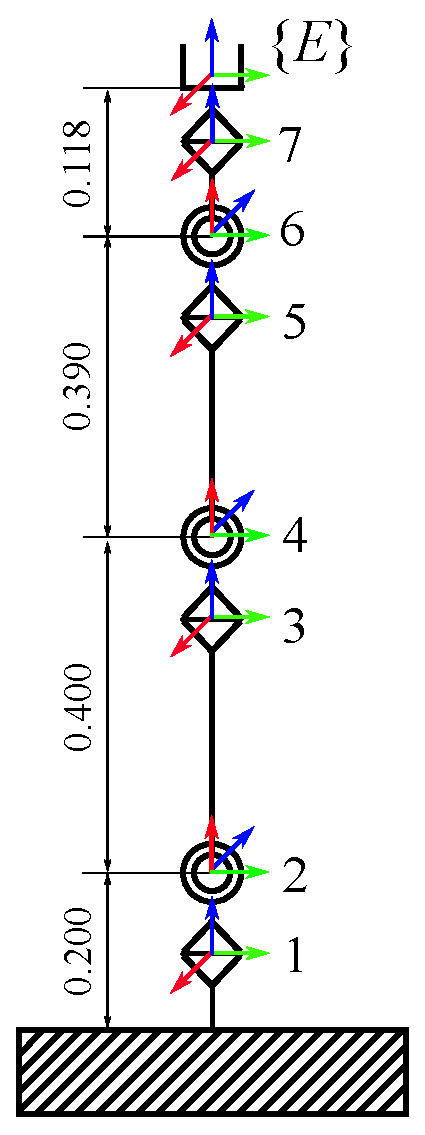
\includegraphics[width=1.0\linewidth]{fig/chapter6/results/spatial/model2.eps}
  \end{minipage}
  \hspace{5em}
  \begin{minipage}[h]{0.22\linewidth}
    \centering
    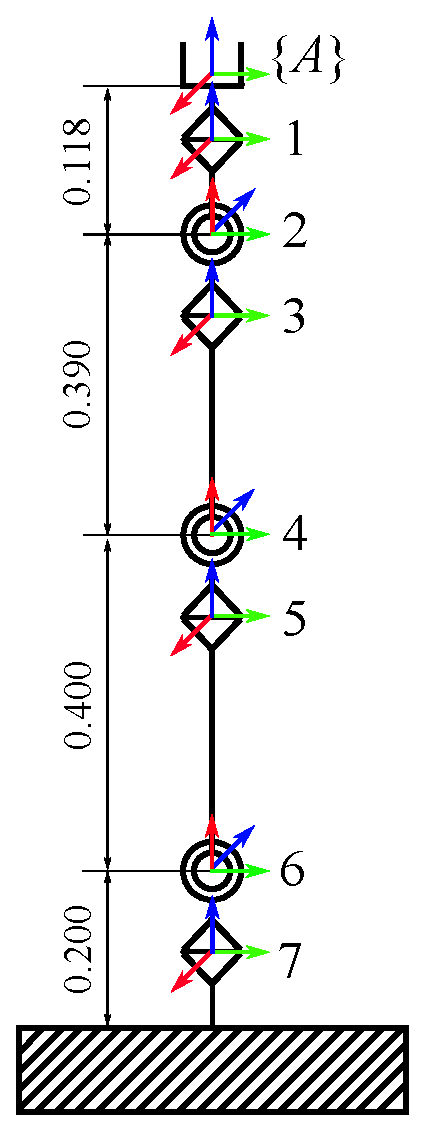
\includegraphics[width=1.0\linewidth]{fig/chapter6/results/spatial/control_model_3.eps}
  \end{minipage}
  \vspace{1em}
  \caption{Simulation model based on the arm of Rollin' Justin.}
  \label{fig:MODEL_JUSTIN}
\end{figure}
% ---------------------------------------------------------------------
%
Next, we verify the performance of the controllers with a seven-DoF redundant manipulator.
The manipulator model is based on the arm of \textit{Rollin' Justin}.
The kinematic structure of the model and its control model for the RNS-based controller are
depicted in \fig{MODEL_JUSTIN}.
With this model, we straightforwardly use the control input describe in \eq{TAU_REF_RNS}.
The model parameters transformation would be done through the same manner in the case of the planar model.
Namely, $\hat{m}_{7}$, $\hbm{I}_{7}$ and $\hat{l}_{3}$ are the constrained link parameters of this model.

%
% ---------------------------------------------------------------------
\begin{figure}[t]
  \centering
  \begin{minipage}[h]{1.0\linewidth}
    \centering
    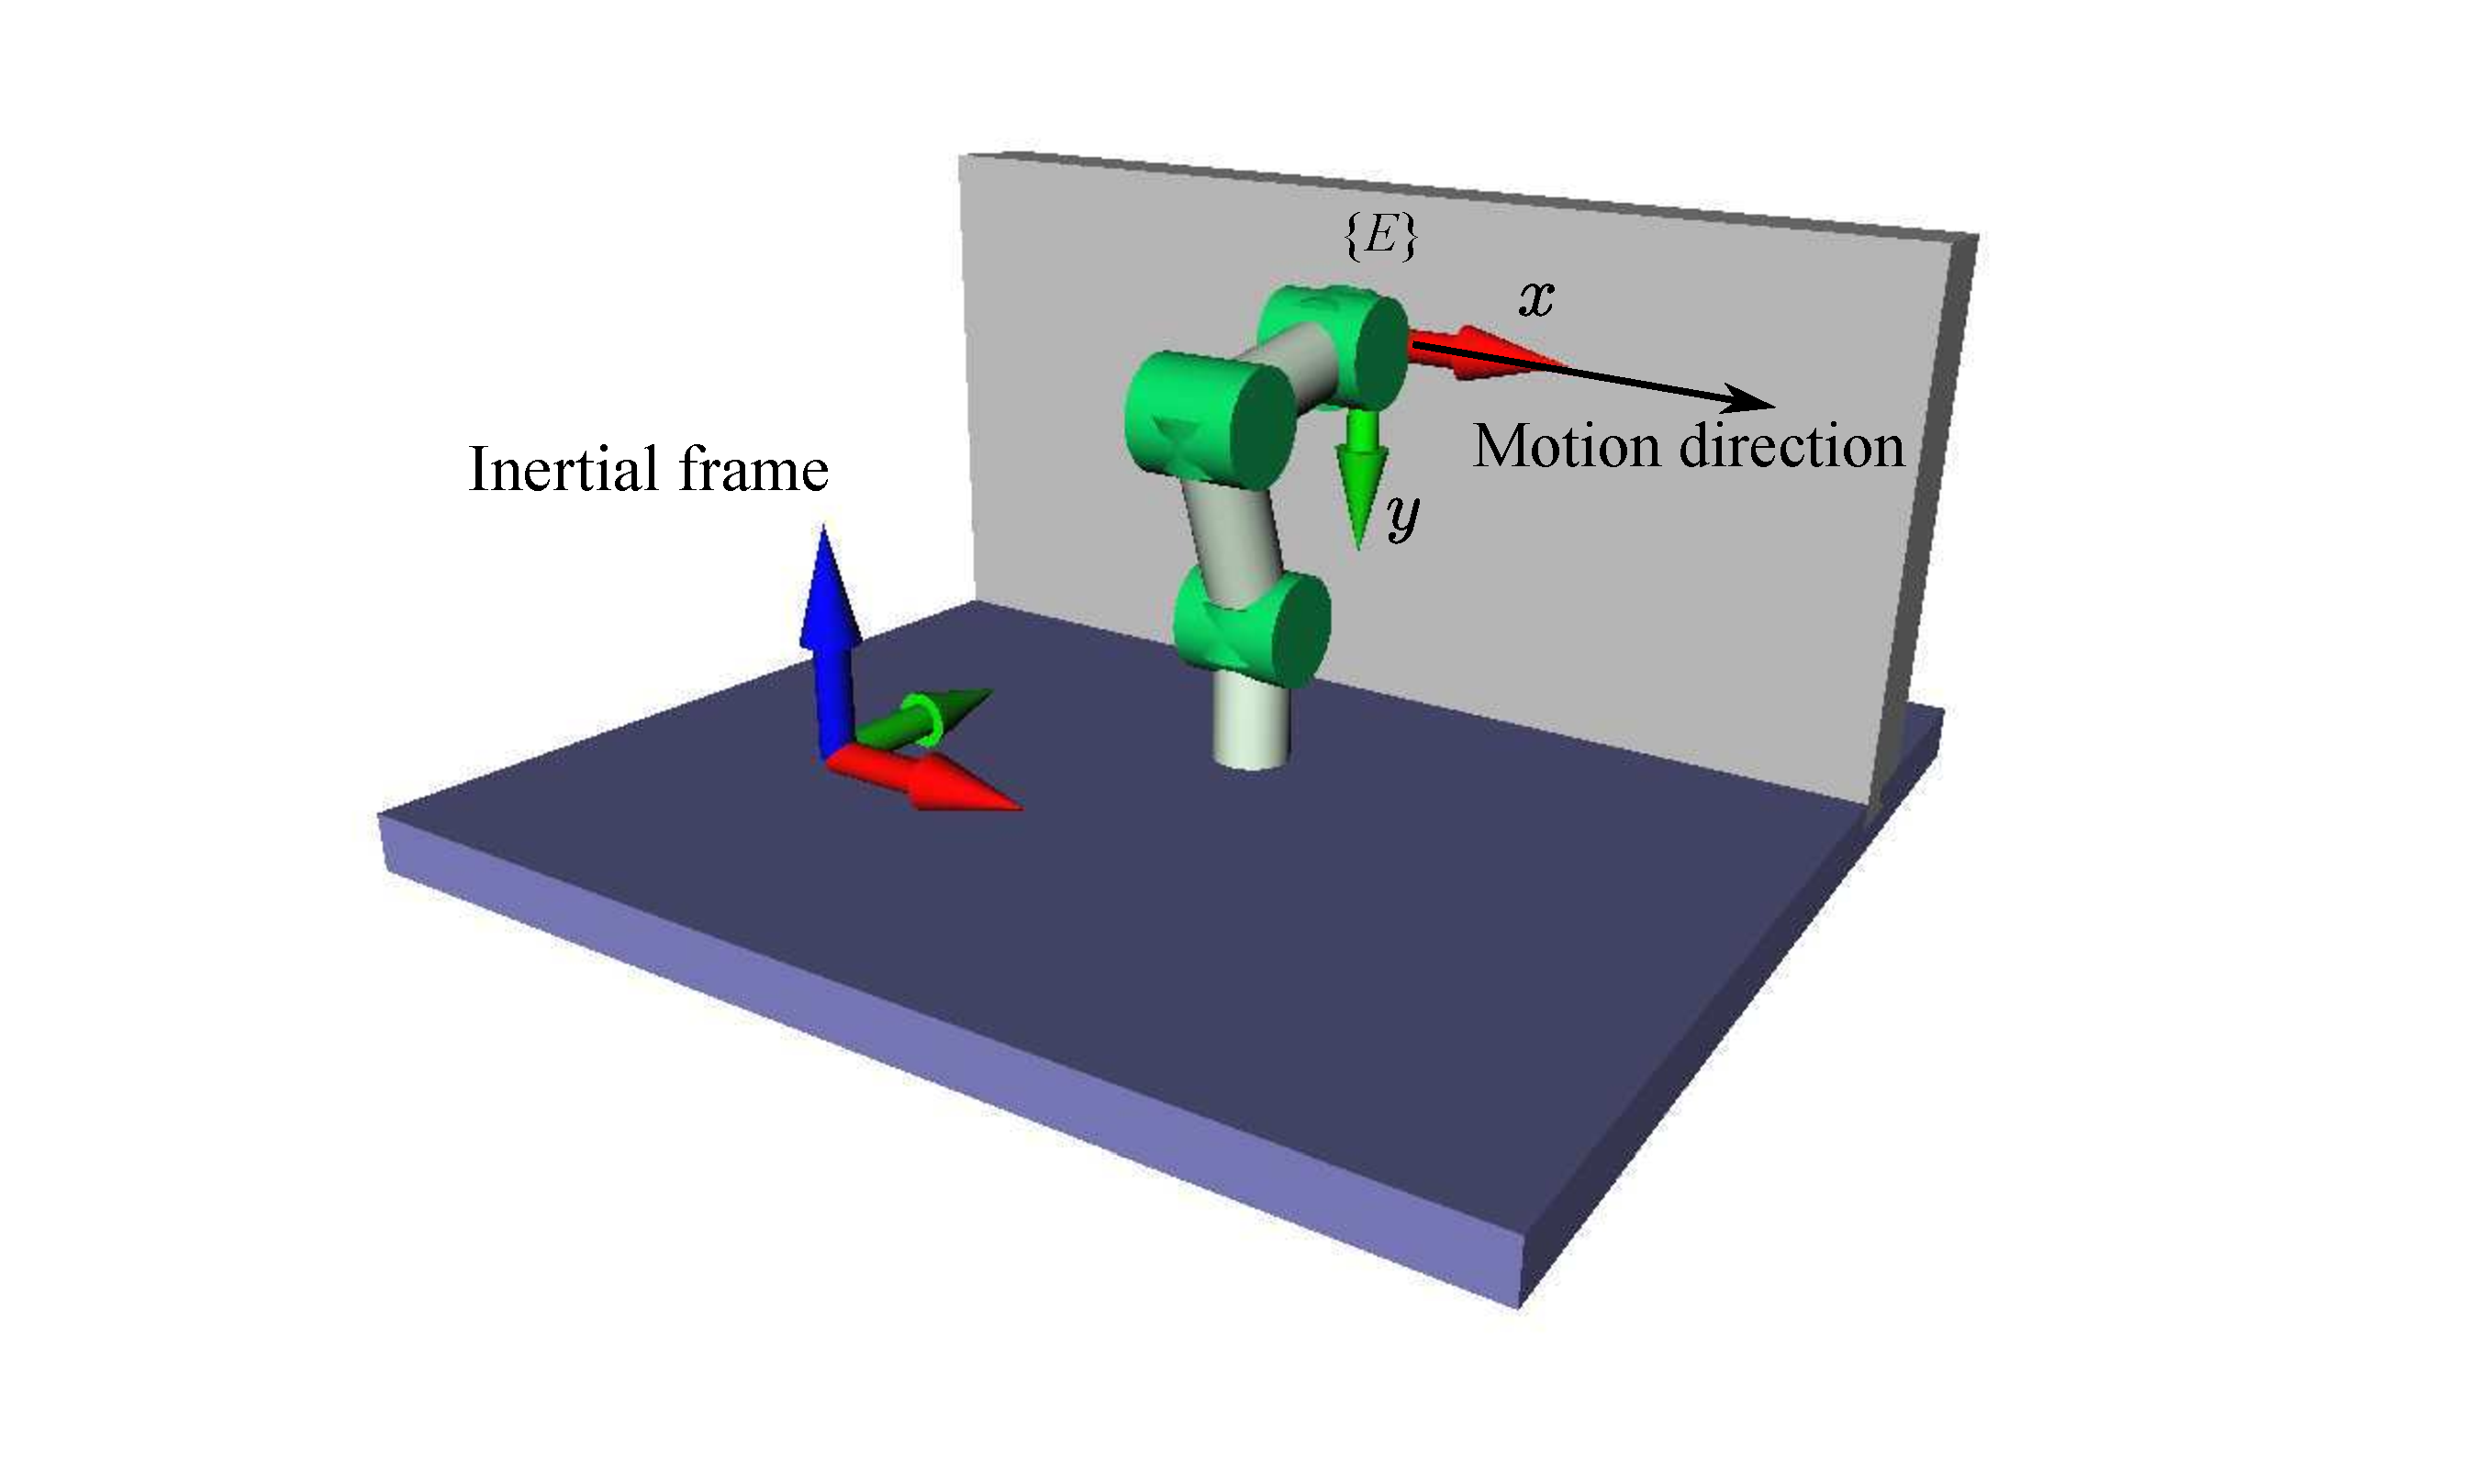
\includegraphics[width=1.0\linewidth]{fig/chapter6/results/spatial/10000.eps}
  \end{minipage}
  \hspace{5em}
  \footnotesize\par{\hspace{2em} Real model \hspace{8em} RNS-based control model}
  \caption{Motion control direction is along $x$ axis,
    while force control direction is along $z$ axis,  in the end-effector frame $\{E\}$.}
  \label{fig:MODEL_JUSTIN_SIM}
\end{figure}
% ---------------------------------------------------------------------
%
The initial configuration is set to $[20~-20~0~100~0~10~0]^{T}\unit{deg}$.
We assume that $z$ direction in $\{E\}$ is the constrained direction due to the wall,
while $x$-$y$ plane in $\{E\}$ is the unconstrained direction as shown in \fig{MODEL_JUSTIN_SIM}.
The desired motion path in the unconstrained direction is defined as a straight line along $x$-axis
to $[0.24~0.43~0.43]^{T}\unit{m}$ via fifth-order spline function.
The desired motion is designed as a repeat motion between the initial position and the final one
during $2.5\unit{s}$, respectively.
The desired force trajectory acting to $z$ axis is defined as a fifth-order spline function during the first second,
with a maximum value set at $10\unit{N}$.
In this case, simulation of the OS formulation is also executed under the same conditions.
Note that, in both cases, orientation of the end-effector is fixed for the sake of simplicity.


%
% ---------------------------------------------------------------------
\begin{figure}[t]
  \centering
  \begin{minipage}[h]{0.40\linewidth}
    \centering
    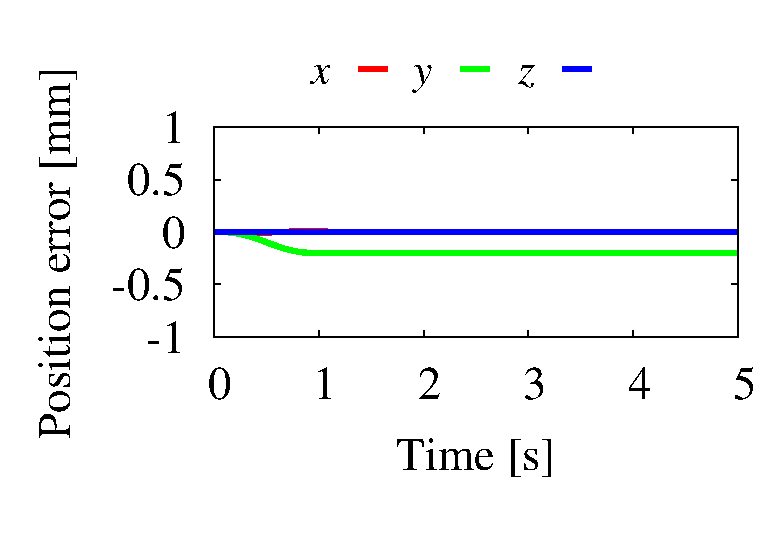
\includegraphics[width=1.0\linewidth]{fig/chapter6/results/spatial/RNS/RNS_U02_pos_err.eps}
  \end{minipage}
  \begin{minipage}[h]{0.40\linewidth}
    \centering
        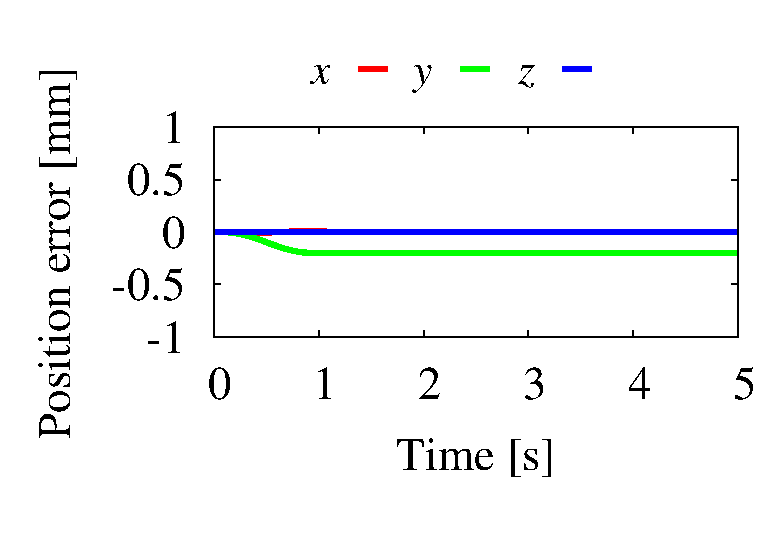
\includegraphics[width=1.0\linewidth]{fig/chapter6/results/spatial/OSF/OSF_U02_pos_err.eps}
  \end{minipage}\\
  \vspace{-3mm}
  \begin{minipage}[h]{0.40\linewidth}
    \centering
    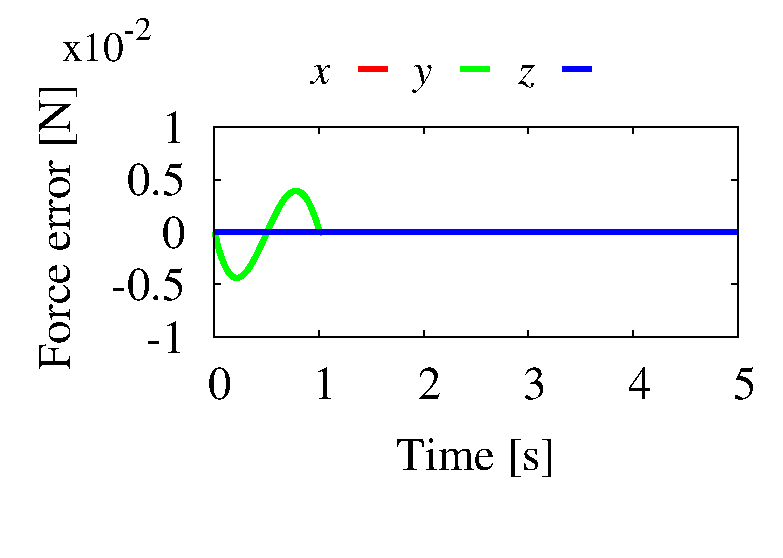
\includegraphics[width=1.0\linewidth]{fig/chapter6/results/spatial/RNS/RNS_U06_force_error.eps}
  \end{minipage}
  \begin{minipage}[h]{0.40\linewidth}
    \centering
    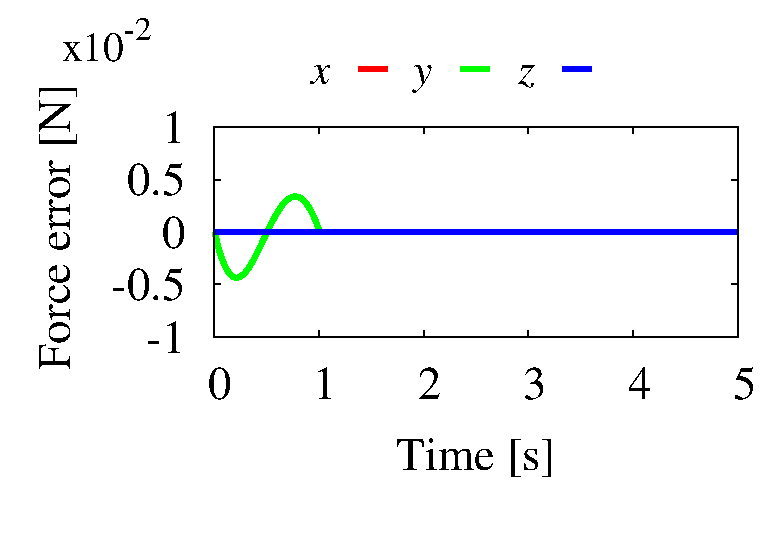
\includegraphics[width=1.0\linewidth]{fig/chapter6/results/spatial/OSF/OSF_U06_force_error.eps}
  \end{minipage}
  \footnotesize\par{RNS-C \hspace{13em} OS-C}
  \vspace{1em}
  \caption{Simulation results of end-effector position and force measured in the inertial frame.}
  \label{fig:RES_MF_7R_TASK}
\end{figure}
% ---------------------------------------------------------------------
%
%
% ---------------------------------------------------------------------
\begin{figure}[t]
  \centering
  \begin{minipage}[h]{0.40\linewidth}
    \centering
    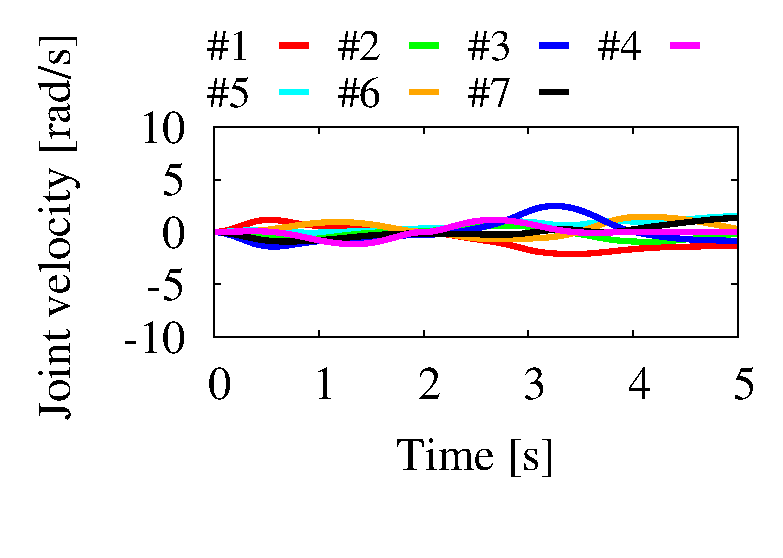
\includegraphics[width=1.0\linewidth]{fig/chapter6/results/spatial/RNS/RNS_X03_Joint_velocity.eps}
  \end{minipage}
  \begin{minipage}[h]{0.40\linewidth}
    \centering
        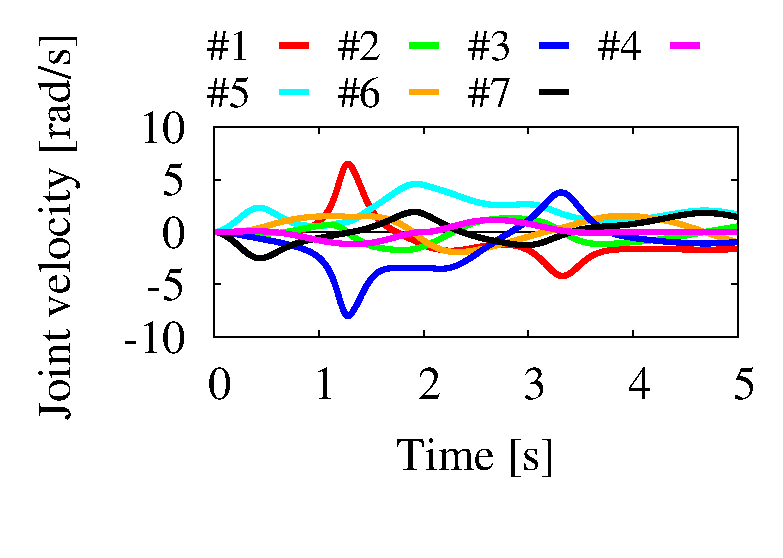
\includegraphics[width=1.0\linewidth]{fig/chapter6/results/spatial/OSF/OSF_X03_Joint_velocity.eps}
  \end{minipage}\\
  \vspace{-2mm}
  \begin{minipage}[h]{0.40\linewidth}
    \centering
    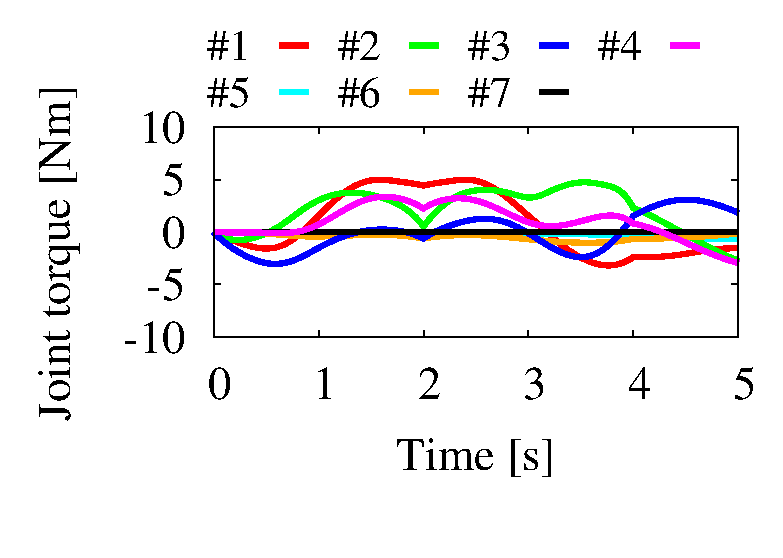
\includegraphics[width=1.0\linewidth]{fig/chapter6/results/spatial/RNS/RNS_U01_joint_torque_1-4.eps}
  \end{minipage}
  \begin{minipage}[h]{0.40\linewidth}
    \centering
    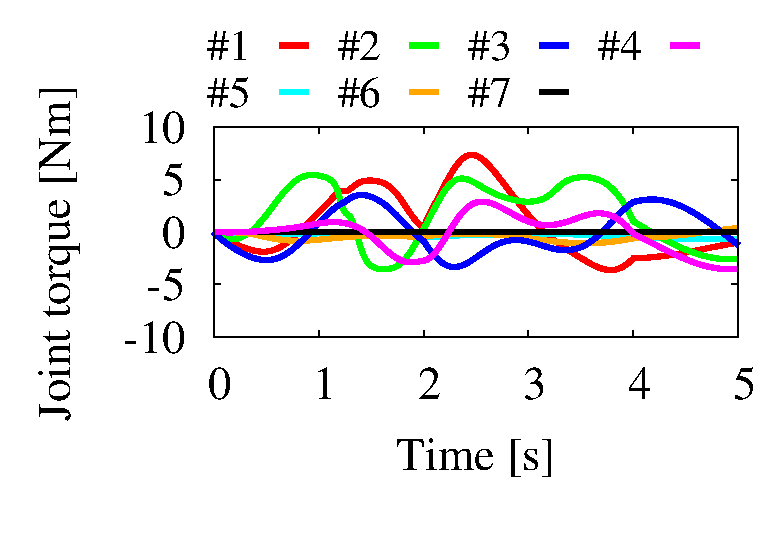
\includegraphics[width=1.0\linewidth]{fig/chapter6/results/spatial/OSF/OSF_U01_joint_torque_1-4.eps}
  \end{minipage}
  \footnotesize\par{RNS-C \hspace{13em} OS-C}
  \vspace{1em}
  \caption{Simulation results of joint-space behavior.}
  \label{fig:RES_MF_7R_JOINT}
\end{figure}
% ---------------------------------------------------------------------
%

Simulation results are displayed in \fig{RES_MF_7R_TASK} and \fig{RES_MF_7R_JOINT}.
These quantities are measured in the inertial frame.
From the results, it becomes apparent that the task-space behavior is almost identical for the two controllers.
On the other hand, there is a different behavior in joint-space, especially joint velocity,
in the same way as the planar case.


%%%%%%%%%%%%%%%%%%%%%
\section{Summary}
%%%%%%%%%%%%%%%%%%%%%
This chapter described motion/force control methods.
From a historical point of view,
we first explained the OS formulation that has been used in various control schemes,
such as hybrid motion/force control and impedance control.
Then, a new introduced motion/force control method based on Reaction Null-Space was presented.
Through numerical simulation with a planar and spatial models,
we verified theirs performance from the perspective of both task-space and joint-space.
It was confirmed that the task-space behaviors were almost identical for the two controllers.
On the other hand,
there was a difference between the two controllers in joint-space;
the amplitude of joint velocities under the RNS-based control can be
reduced smaller than that under the OS formulation.




%**********************************************************************


%
%
%%% Local Variables:
%%% mode: latex
%%% TeX-master: "./main"
%%% End: